
%\documentclass[mathserif]{beamer}
\documentclass[handout]{beamer}
%\usetheme{Goettingen}
%\usetheme{Warsaw}
\usetheme{Singapore}



%\usetheme{Frankfurt}
%\usetheme{Copenhagen}
%\usetheme{Szeged}
%\usetheme{Montpellier}
%\usetheme{CambridgeUS}
%\usecolortheme{}
%\setbeamercovered{transparent}
\usepackage[english, activeacute]{babel}
\usepackage[utf8]{inputenc}
\usepackage{amsmath, amssymb}
\usepackage{dsfont}
\usepackage{graphics}
\usepackage{cases}
\usepackage{graphicx}
\usepackage{pgf}
\usepackage{epsfig}
\usepackage{amssymb}
\usepackage{multirow}	
\usepackage{amstext}
\usepackage[ruled,vlined,lined]{algorithm2e}
\usepackage{amsmath}
\usepackage{epic}
\usepackage{epsfig}
\usepackage{fontenc}
\usepackage{framed,color}
\usepackage{palatino, url, multicol}
%\algsetup{indent=2em}
\newcommand{\factorial}{\ensuremath{\mbox{\sc Factorial}}}
\newcommand{\BIGOP}[1]{\mathop{\mathchoice%
{\raise-0.22em\hbox{\huge $#1$}}%
{\raise-0.05em\hbox{\Large $#1$}}{\hbox{\large $#1$}}{#1}}}
\newcommand{\bigtimes}{\BIGOP{\times}}
\vspace{-0.5cm}
\title{Natural Language Processing \\ Sequence to Sequence Models and Attention}
\vspace{-0.5cm}
\author[Felipe Bravo Márquez]{\footnotesize
%\author{\footnotesize  
 \textcolor[rgb]{0.00,0.00,1.00}{Felipe Bravo-Marquez}} 
  
 

\date{\today}

\begin{document}
\begin{frame}
\titlepage


\end{frame}




\begin{frame}{Language Models and Language Generation}
\begin{scriptsize}
\begin{itemize}
\item Language modeling is the task of assigning a probability to sentences in a language.
\item Example: what is the probability of seeing the sentence ``the lazy dog barked loudly''?
\item The task can be formulated as the task of predicting the probability of seeing a word conditioned on previous words:
\begin{displaymath}
 P(w_i | w_1, w_2, \cdots, w_{i-1}) = \frac{P(w_1, w_2, \cdots, w_{i-1}, w_i)}{P(w_1, w_2, \cdots, w_{i-1})}  
\end{displaymath}

\end{itemize}
\end{scriptsize}
\end{frame}


\begin{frame}{Language Models and Language Generation}
\begin{scriptsize}
\begin{itemize}
\item  RNNs can be used to train language models by tying the output at time $i$ with its input at time $i + 1$ .
\item This network can be used to generate sequences of words or random sentences.
\item Generation process: predict a probability distribution over the first word conditioned on the start symbol, and draw a random word according to the predicted
distribution.

\item Then predict a probability distribution over the second word conditioned on the first, and so on, until predicting the end-of-sequence $</$s$>$ symbol.
\end{itemize}
\end{scriptsize}
\end{frame}


\begin{frame}{Language Models and Language Generation}
\begin{scriptsize}
\begin{itemize}
\item After predicting a distribution over the next output symbols $P(t_i = k | t_{1:i-1})$, a token $t_i$ is chosen and its corresponding embedding vector is fed as the input to the next step.
         \begin{figure}[h]
        	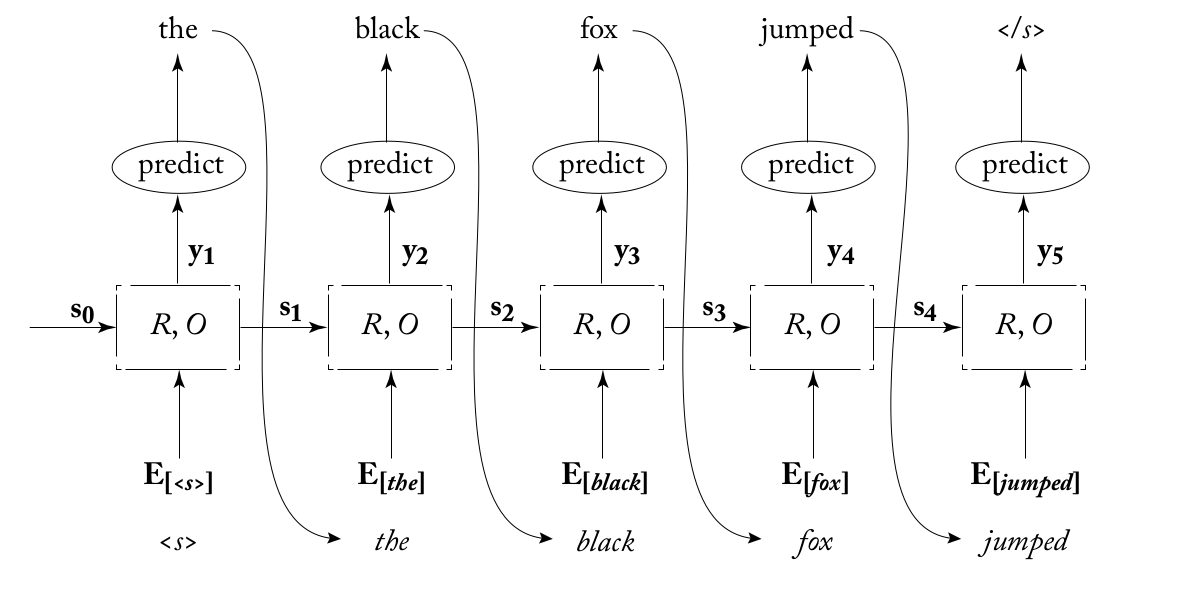
\includegraphics[scale = 0.25]{pics/generator.png}
        \end{figure}  
        
\item Teacher-forcing: during \textbf{training} the generator is fed with the ground-truth previous word even if its own prediction put a small probability mass on it. 
\item It is likely that the generator would have generated a different word at this state in \textbf{test time}.        
\end{itemize}
        
        
\end{scriptsize}
\end{frame}




\begin{frame}{Sequence to Sequence Problems}
\begin{scriptsize}
Nearly any task in NLP can be formulated as a sequence to sequence (or conditioned generation) task i.e., generate output sequences from input ones. Input and output sequences can have different lengths.
\begin{itemize}
\item Machine Translation: source language to target language.
\item Summarization: long text to short text.
\item Dialogue (chatbots): previous utterances to next utterance.
\end{itemize}
\end{scriptsize}
\end{frame}



\begin{frame}{Conditioned Generation}
\begin{scriptsize}
\begin{itemize}
\item While using the RNN as a generator is a cute exercise for demonstrating its strength, the power of RNN generator is really revealed when moving to a conditioned generation or encoder-decoder framework.
\item Core idea: using two RNNs.
\item Encoder: One RNN is used to encode the source input into a vector $\overrightarrow{c}$.
\item Decoder: Another RNN is used to decode the encoder's output and generate the target output.
\item At each stage of the generation process the context vector $\overrightarrow{c}$ is concatenated to the input $\hat{t}_j$ and the concatenation is fed into the RNN.
\end{itemize}
\end{scriptsize}
\end{frame}


\begin{frame}{Encoder Decoder Framework}
         \begin{figure}[h]
        	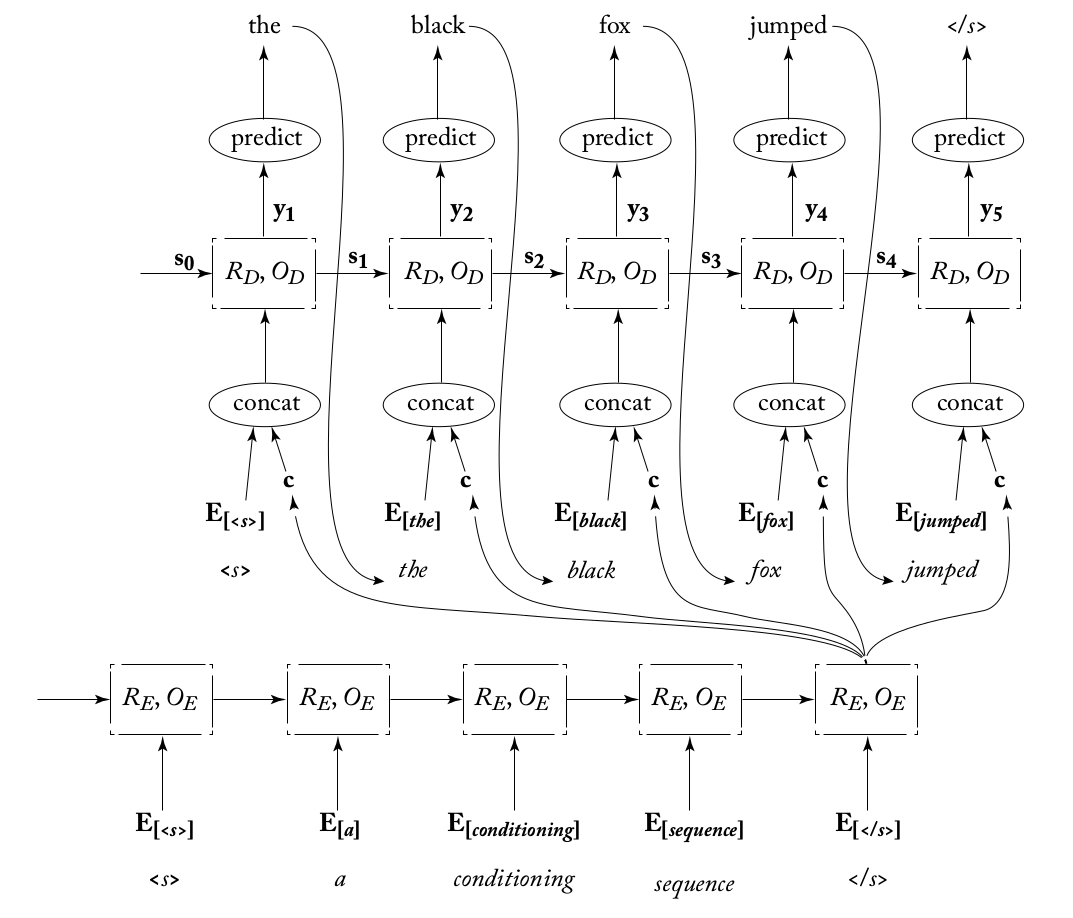
\includegraphics[scale = 0.32]{pics/seqseq.png}
        \end{figure}  
\end{frame}




\begin{frame}{Conditioned Generation}
\begin{scriptsize}
\begin{itemize}
\item This setup is useful for mapping sequences of length $n$ to sequences of length $m$.
\item The encoder summarizes the source sentence as a vector $\vec{c}$.
\item The decoder RNN is then used to predict (using a language modeling objective) the target sequence words conditioned on the previously predicted words as well as the encoded sentence $\vec{c}$.
\item The encoder and decoder RNNs are trained jointly.
\item The supervision happens only for the decoder RNN, but the gradients are propagated all the way back to the encoder RNN.
\end{itemize}
\end{scriptsize}
\end{frame}


\begin{frame}{Sequence to Sequence Training Graph}
         \begin{figure}[h]
        	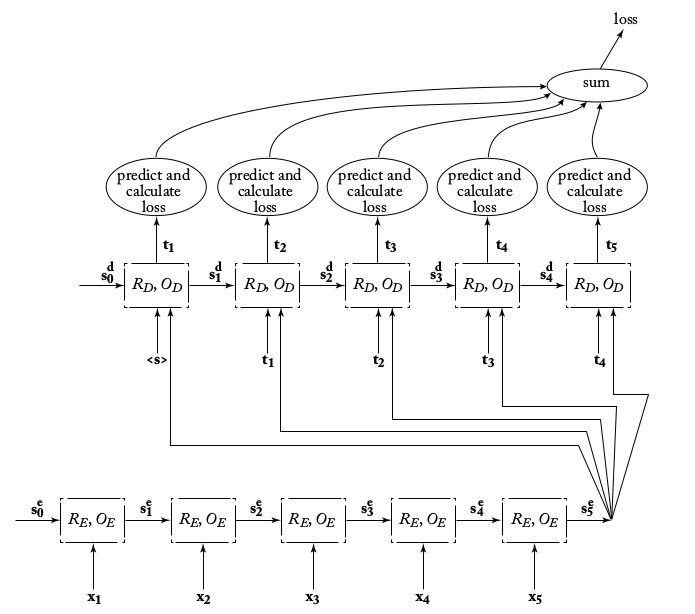
\includegraphics[scale = 0.35]{pics/seq2se2train.png}
        \end{figure}  
    
\end{frame}




\begin{frame}{Neural Machine Translation}
         \begin{figure}[h]
        	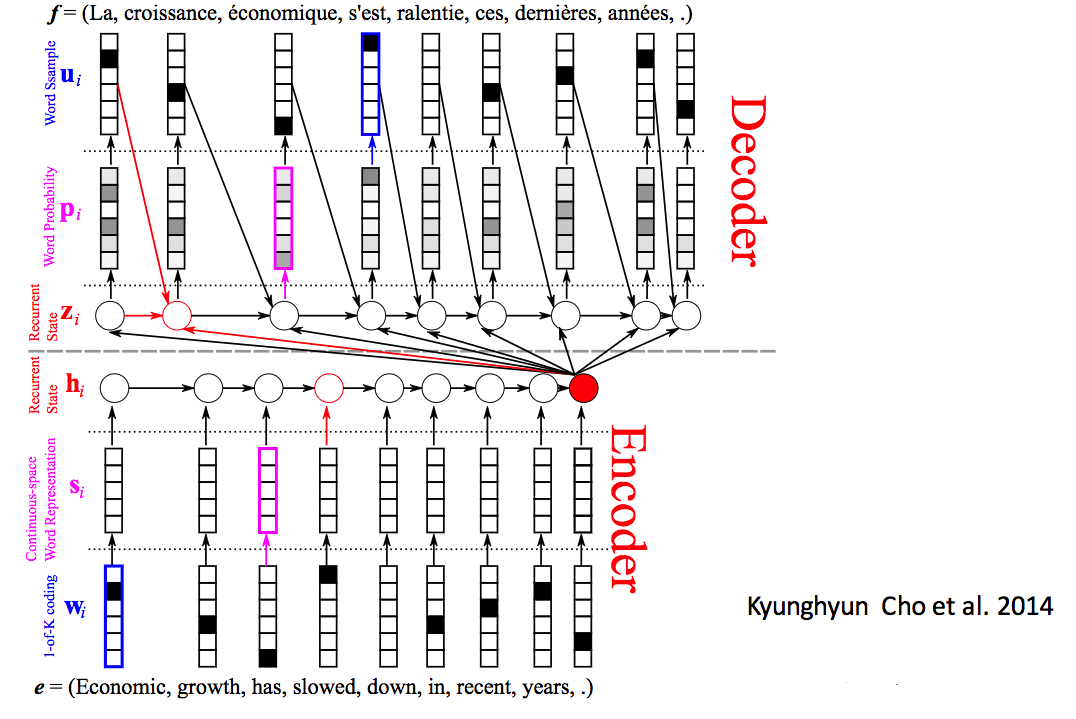
\includegraphics[scale = 0.25]{pics/mt.png}
        \end{figure}  
\end{frame}


\begin{frame}{Machine Translation BLEU progress over time}
         \begin{figure}[h]
        	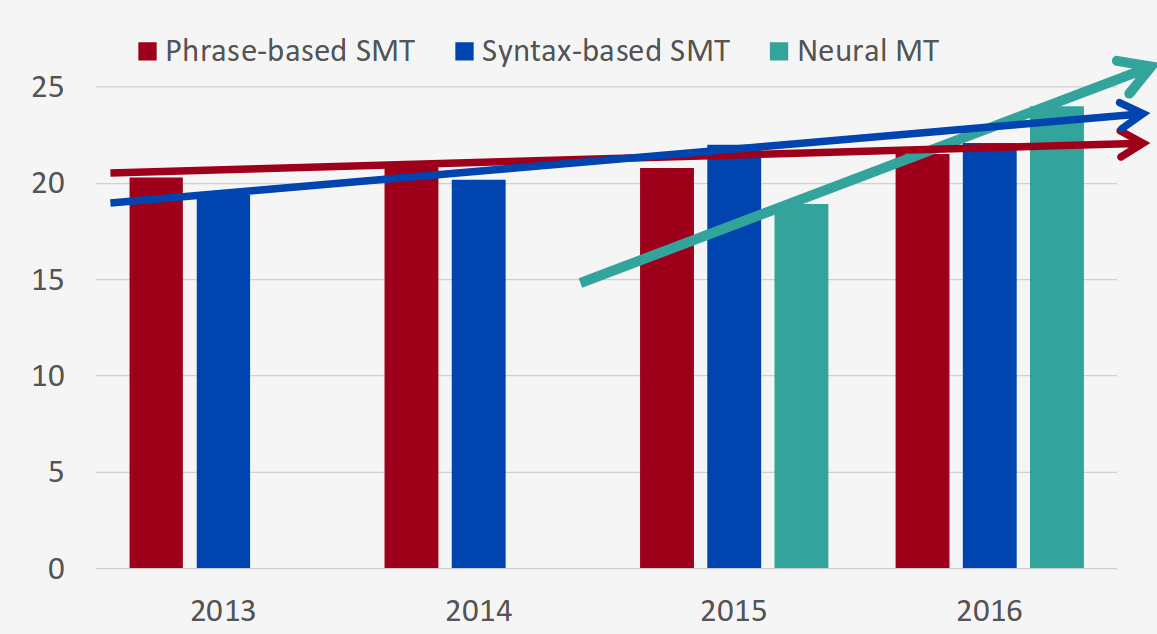
\includegraphics[scale = 0.35]{pics/nmt_progress.png}
        \end{figure}  
[Edinburgh En-De WMT]        
\footnotetext{source: \url{http://www.meta-net.eu/events/meta-forum-2016/slides/09_sennrich.pdf}}      
\end{frame}

\begin{frame}{Decoding Approaches}
\begin{scriptsize}
\begin{itemize}
\item The decoder aims to generate  the output sequence with maximal score (or maximal probability), i.e., such that $\sum_{i=1}^{n}P(\hat{t}_i | \hat{t}_{1:i-1})$ is maximized. 
\item The non-markovian nature of the RNN means that the probability function cannot be decomposed into factors that allow for exact search using standard dynamic programming.
\item Exact search: finding the optimum sequence requires evaluating every possible sequence (computationally prohibitive).
\item Thus, it only makes sense to solving the optimization problem above approximately.
\item Greedy search: choose the highest scoring prediction (word) at each step.
\item This may result in sub-optimal overall probability leading to
prefixes that are followed by low-probability events.

\end{itemize}
        
        
\end{scriptsize}
\end{frame}


\begin{frame}{Greedy Search}
        
         \begin{figure}[h]
        	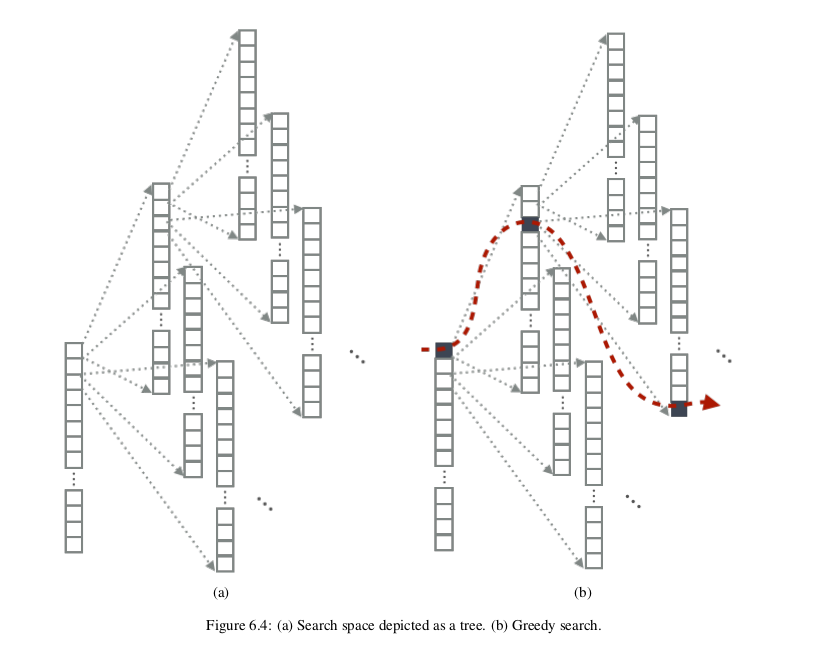
\includegraphics[scale = 0.3]{pics/greedysearch.png}
        \end{figure}        
        
        
        
\footnotetext{Source: \cite{cho2015natural}}
        
\end{frame}



\begin{frame}{Beam Search}
\begin{scriptsize}
\begin{itemize}
\item Beam search interpolates between the exact search and the greedy search by changing the size $K$ of hypotheses maintained throughout the search procedure \cite{cho2015natural}.
\item The Beam search algorithm works in stages.
\item  We first pick the $K$ starting words with the highest probability 
\item At each step, each candidate sequence is expanded with all possible next steps. 
\item Each candidate step is scored. 
\item The $K$ sequences with the most likely probabilities are retained and all other candidates are pruned. 
\item The search process can halt for each candidate separately either by reaching a maximum length, by reaching an end-of-sequence token, or by reaching a threshold likelihood.
\item The sentence with the highest overall probability is selected.
\end{itemize}
        
\footnotetext{More info at: \url{https://machinelearningmastery.com/beam-search-decoder-natural-language-processing/}}        
\end{scriptsize}
\end{frame}





\begin{frame}{Conditioned Generation with Attention}
\begin{scriptsize}
\begin{itemize}
\item In the encoder-decoder networks the input sentence is encoded into a single vector, which is then used as a conditioning context for an RNN-generator. 
\item This architectures forces the encoded vector $\vec{c}$ to contain all the information required for generation.
\item It doesn't work well for long sentences!
\item It also requires the generator to be able to extract this information from the fixed-length vector.
\item ``You can't cram the meaning of a whole \%\&!\$\# sentence into a single \$\&!\#* vector!'' -Raymond Mooney
\item This architecture can be can be substantially improved (in many cases) by the addition of an attention mechanism.
\item The attention mechanism attempts to solve this problem by allowing the decoder to “look back” at the encoder’s hidden states based on its current state. 
\end{itemize}
\end{scriptsize}
\end{frame}



\begin{frame}{Conditioned Generation with Attention}
\begin{scriptsize}
\begin{itemize}
\item The input sentence (a length $n$ input sequence $\vec{x}_{1:n}$) is encoded using a biRNN as a sequence of vectors $\vec{c}_{1:n}$.  
\item The decoder uses a soft attention mechanism in order to decide on which parts of the encoding input it should focus. 
\item At each stage $j$ the decoder sees a weighted average of the vectors $\vec{c}_{1:n}$ , where the attention weights ($\vec{\alpha}^j$) are chosen by the attention mechanism.
\begin{displaymath}
\vec{c}^j = \sum_{i=1}^{n} \vec{\alpha}_{[i]}^{j}\cdot \vec{c}_i 
\end{displaymath}
\item The elements of $\vec{\alpha}^j$ are all positive and sum to one.



\end{itemize}
\end{scriptsize}
\end{frame}





\begin{frame}{Conditioned Generation with Attention}
\begin{scriptsize}
\begin{itemize}
\item Unnormalized attention weights ($\bar{\alpha}_{[i]}^j$)  are produced taking into account the decoder state at time $j$ ($\vec{s}_j$) and each of the vectors $\vec{c}_i$.
\item They can be obtained in various ways, basically any differentiable function returning a scalar out of two vectors $\vec{s}_j$ and  $\vec{c}_i$ could be employed. 
\item The simplest approach is a dot product:  $\bar{\alpha}_{[i]}^j = \vec{s}_j \cdot \vec{c}_i$. 
\item The one we will use in these slides is Additive attention, which uses a Multilayer Perceptron: $\bar{\alpha}_{[i]}^j = MLP^{att}([\vec{s}_j;\vec{c}_i]) = \vec{v} \cdot \operatorname{tanh}([\vec{s}_j;\vec{c}_i]U +\vec{b})$

\end{itemize}
\end{scriptsize}
\end{frame}


\begin{frame}{Conditioned Generation with Attention}
\begin{scriptsize}
\begin{itemize}
\item These unnormalized weights are then normalized into a probability distribution using the softmax function.

\begin{figure}[h]
        	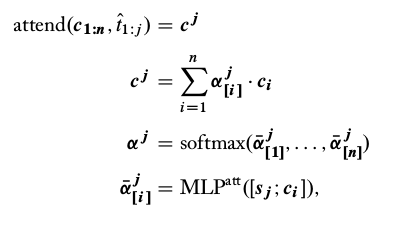
\includegraphics[scale = 0.35]{pics/atten_formula.png}
        \end{figure}  

        
                

\item The encoder, decoder, and attention mechanism are all trained jointly in order to play well with each other.


\end{itemize}
\end{scriptsize}
\end{frame}





\begin{frame}{Attention}
         \begin{figure}[h]
        	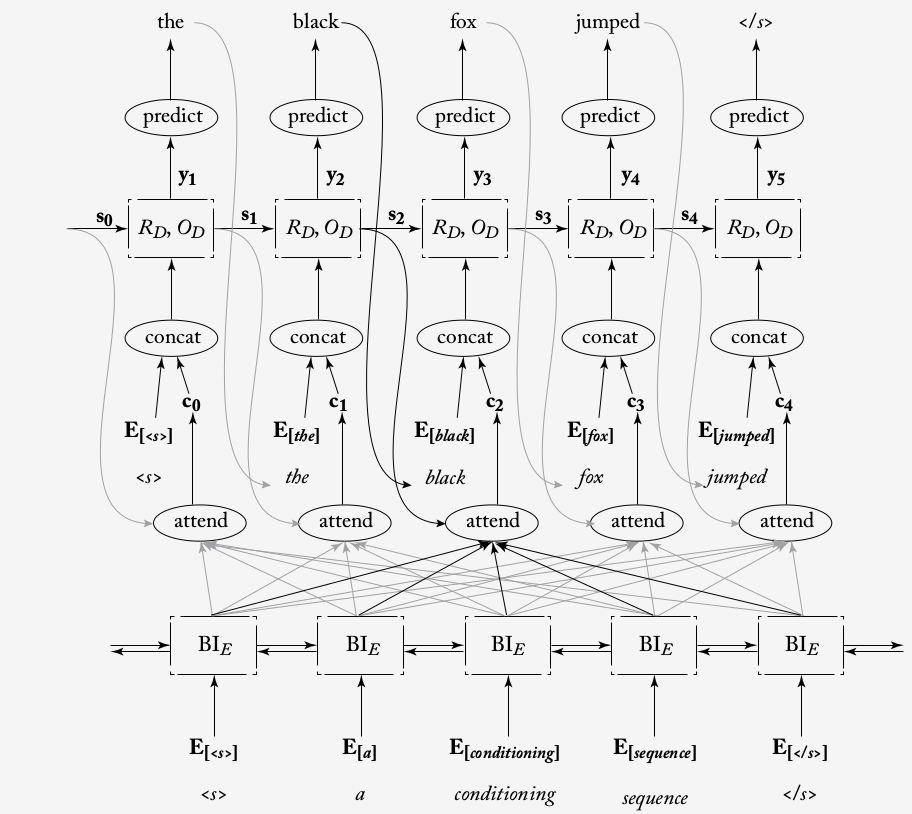
\includegraphics[scale = 0.35]{pics/encdecattention.png}
        \end{figure}  
\end{frame}



\begin{frame}{Conditioned Generation with Attention}
\begin{scriptsize}
The entire sequence-to-sequence generation with attention is given by:

\begin{figure}[h]
        	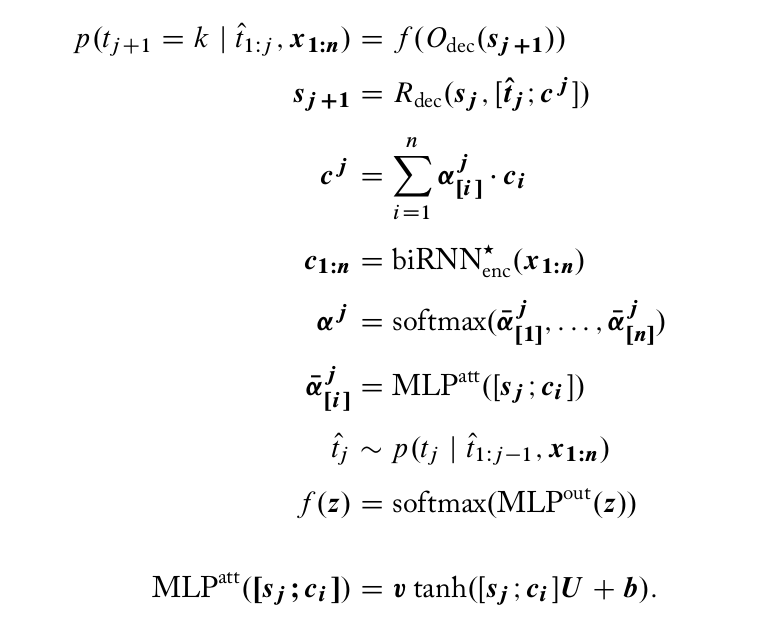
\includegraphics[scale = 0.3]{pics/attentionformula.png}
        \end{figure}  

        
                
\end{scriptsize}
\end{frame}



\begin{frame}{Conditioned Generation with Attention}
\begin{scriptsize}
\begin{itemize}
\item Why use the biRNN encoder to translate the conditioning sequence $\vec{x}_{1:n}$  into the context vectors $\vec{c}_{1:n}$?
\item Why we just don't attend directly on the inputs (word embeddings) $MLP^{att}([\vec{s}_j;\vec{x}_i])$?
\item We could, but we get important benefits from the encoding process.
\item First, the biRNN vectors $\vec{c}_i$ represent the items $\vec{x}_i$ in their sentential context.
\item Sentential context: a window focused around the input item $\vec{x}_i$ and not the item itself.
\item Second, by having a trainable encoding component that is trained jointly with the decoder, the encoder and decoder evolve together.
\item Hence, the network can learn to encode relevant properties of the input that are useful for decoding, and that may not be present at the source sequence $\vec{x}_{1:n}$ directly.
\end{itemize}
\end{scriptsize}
\end{frame}


\begin{frame}{Attention and Word Alignments}
\begin{scriptsize}
\begin{itemize}
\item In the context of machine translation, one can think of $MLP^{att}$ as computing a soft alignment between the current decoder state $\vec{s}_j$ (capturing the recently produced foreign words) and each of the source sentence components $\vec{c}_i$.


\end{itemize}


         \begin{figure}[h]
        	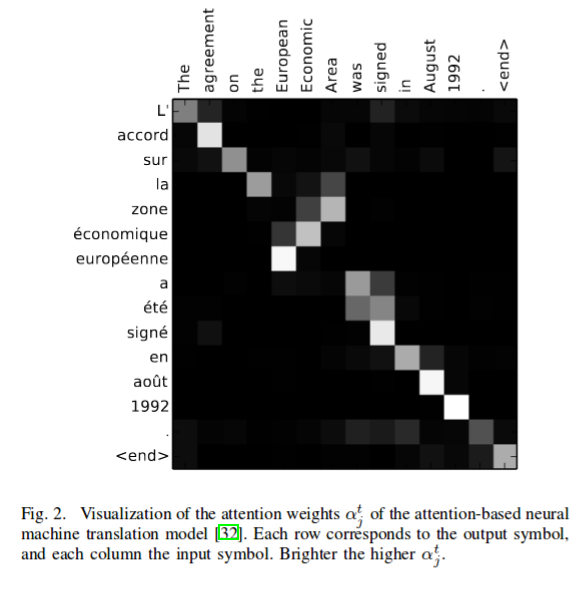
\includegraphics[scale = 0.28]{pics/attention-alignment.png}
        	\caption{Source: \cite{cho2015describing}}
        \end{figure}  


\end{scriptsize}
\end{frame}



\begin{frame}{Other types of Attention}
\begin{scriptsize}

       \begin{figure}[h]
        	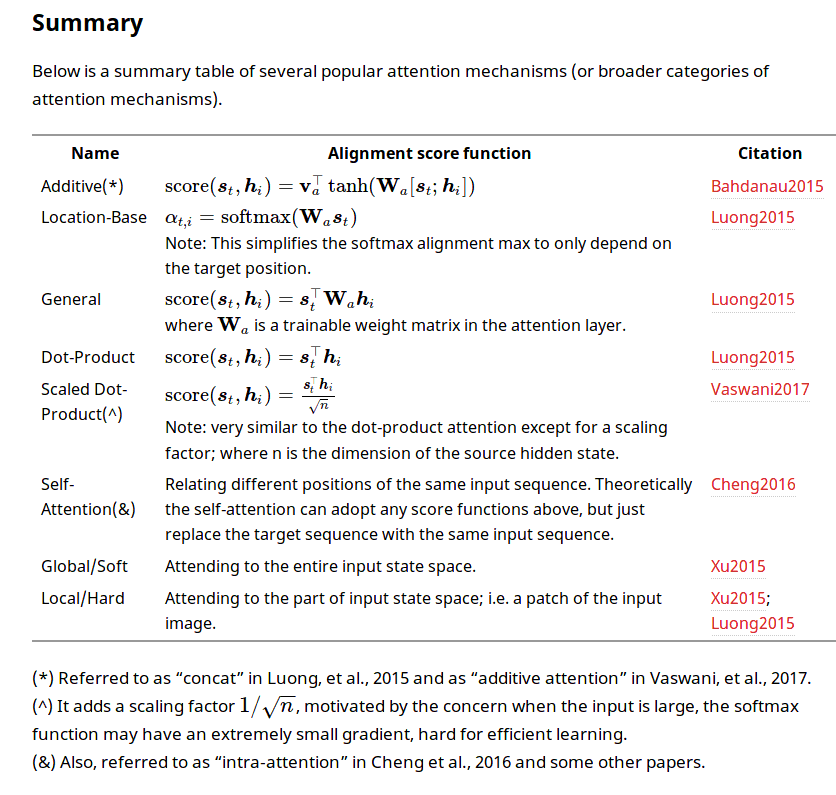
\includegraphics[scale = 0.32]{pics/types_of_attention.png}
        	\caption{Source: \url{https://lilianweng.github.io/lil-log/2018/06/24/attention-attention.html}}
        \end{figure}  


\end{scriptsize}
\end{frame}


\begin{frame}
\frametitle{Questions?}
%\vspace{1.5cm}
\begin{center}\LARGE Thanks for your Attention!\\ \end{center}



\end{frame}

\begin{frame}[allowframebreaks]\scriptsize
\frametitle{References}
\bibliography{bio}
\bibliographystyle{apalike}
%\bibliographystyle{flexbib}
\end{frame}  


%%%%%%%%%%%%%%%%%%%%%%%%%%%

\end{document}
